\subsection{Configuración de \gls{term:kibana}}
\label{configuracion-de-kibana}

En el \autoref{cap4} hemos hablado de cómo usamos \gls{term:elasticsearch} para
almacenar los datos obtenidos de Logs. El siguiente paso es usar
\gls{term:kibana} para poder visualizar los datos almacenados en
\gls{term:elasticsearch}.

Usaremos \gls{term:kibana} a través de la imagen de \gls{term:docker} oficial.
Esta imagen provee varios métodos para configurar \gls{term:kibana}. El enfoque
convencional es proveer un archivo \lstinline{kibana.yml}, pero también es
posible utilizar variables de ambiente para definir las opciones.

Agregamos las siguientes líneas al \lstinline{docker-compose.yml}:

\begin{lstlisting}
services:
  ...
  kibana:
    image: kibana
    restart: always
    ports:
      - "5601:5601"
    environment:
      - ELASTICSEARCH_URL=http://elasticsearch:9200
    networks:
      - lognet
\end{lstlisting}

Podemos acceder a la aplicación \gls{acro:web} de \gls{term:kibana}
(\autoref{fig:kibana-default}) a través del puerto 5601. Todo lo que uno
necesita es apuntar el navegador \gls{acro:web} a la máquina en la cual
\gls{term:kibana} está siendo ejecutada y especificar el número de puerto.

\begin{figure}
  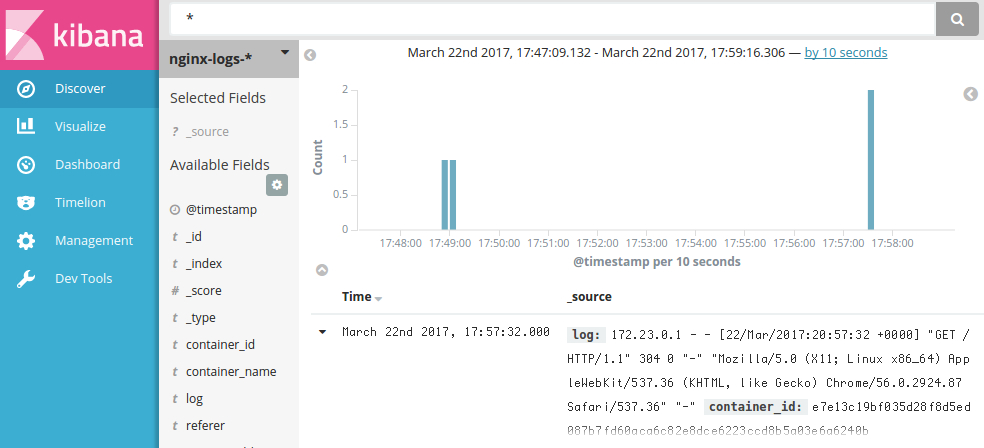
\includegraphics[width=\linewidth]{src/images/05-capitulo-5/kibanadefault.jpg}
  \caption{Cliente de \gls{term:kibana} al acceder al puerto 5601}
  \label{fig:kibana-default}
\end{figure}

Cuando se accede a \gls{term:kibana}, la página de descubrimiento se carga por
defecto con el patrón del índice por defecto seleccionado. El filtro de tiempo
es fijado a los últimos 15 minutos y la consulta de búsqueda es colocada para
traer todos los resultados.

Es posible alcanzar el estado de página del servidor de \gls{term:kibana}
navegando a la dirección \lstinline{localhost:5601/status}. La página de estado
(\autoref{fig:kibana-status}) muestra información acerca del uso de recursos
del servidor y lista los plugins instalados.

\begin{figure}
  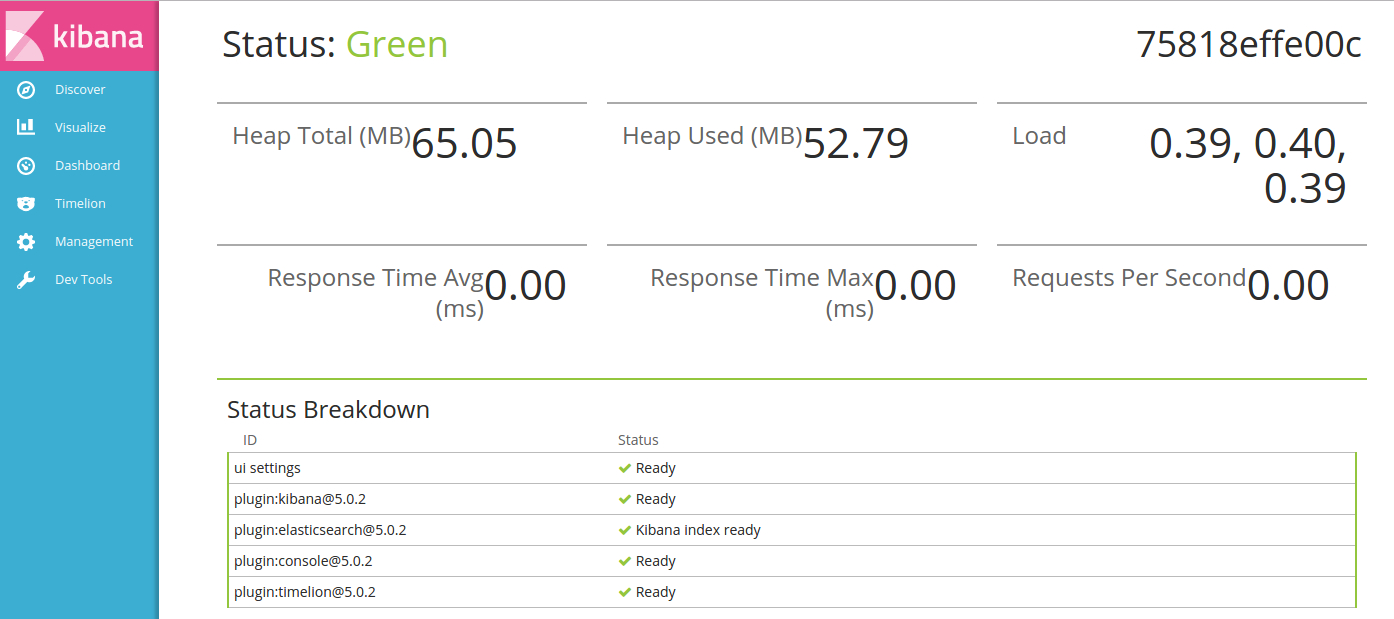
\includegraphics[width=\linewidth]{src/images/05-capitulo-5/kibanastatus.jpg}
  \caption{Vista del estado del servidor desde \gls{term:kibana}}
  \label{fig:kibana-status}
\end{figure}


Para poder comenzar a usar \gls{term:kibana}, debemos indicarle los índices de
\gls{term:elasticsearch} que queremos explorar. La primera vez que se accede a
\gls{term:kibana}, se solicita al usuario definir un patrón que coincida con
los nombres de uno o más índices. Una vez hecho esto ya podemos empezar a
explorar datos.



Con \gls{term:kibana} es posible explorar los datos de forma interactiva a
través de la página de descubrimiento. Desde esta página se tiene acceso a cada
documento en cada índice que coincida con un patrón de nombres de índices
seleccionado.

De esta forma, es posible enviar consultas de búsquedas, filtrar los resultados
de las búsquedas y visualizar datos de los documentos. Además se pueden ver los
números de documentos que coinciden con la consulta de búsqueda y obtener
estadísticas de valores de campos.

\begin{figure}
  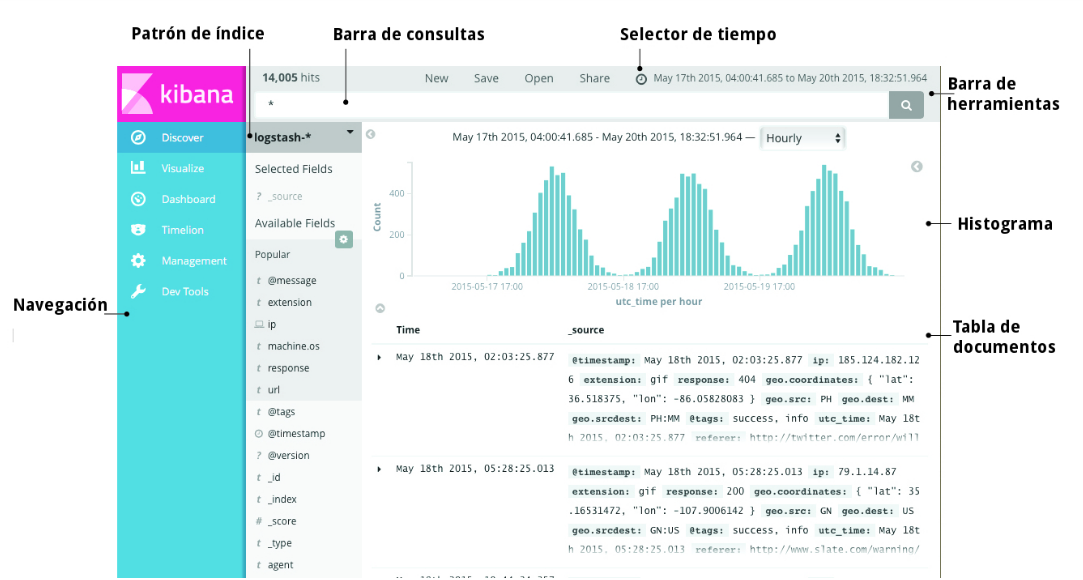
\includegraphics[width=\linewidth]{src/images/05-capitulo-5/kibana-ux.png}
  \caption{Explicación de las partes de la interfaz de \gls{term:kibana}}
  \label{fig:kibana-ux}
\end{figure}


Si un campo de tiempo es configurado para el patrón de índice seleccionado, la
distribución de documentos en el tiempo es mostrada en un \gls{term:histograma}
en la parte de arriba de la página.

\gls{term:kibana} permite crear visualizaciones de datos en los índices de
\gls{term:elasticsearch}, y con ellas construir tableros que muestren
visualizaciones relacionadas.

Las visualizaciones de \gls{term:kibana} están basadas en consultas de
\gls{term:elasticsearch}. Al usar una serie de agregaciones de
\gls{term:elasticsearch} para extraer y procesar datos, se pueden crear
gráficos que muestren tendencias, picos y caídas que puede ser importante
conocer.

Es posible crear visualizaciones de distintos tipos. Algunos de estos tipos son:


\begin{itemize}

  \item \textbf{Gráficos de área:}
  Visualizar la contribución total de varias series distintas.

  \item \textbf{Tabla de datos:}
  Mostrar datos crudos de una agregación compuesta.

  \item \textbf{Gráfico de líneas:}
  Comparar diferentes series.

  \item \textbf{Métrica:}
  Muestra un único número.

  \item \textbf{Gráfico de torta:}
  Comparar la contribución de cada fuente.

  \item \textbf{Nube de etiquetas:}
  Mostrar palabras de forma que el tamaño de la palabra corresponde con su importancia.

  \item \textbf{Serie de tiempo:}
  Computar y combinar datos de múltiples conjuntos de datos de tipo serie de tiempo.

  \item \textbf{Gráfico de barras vertical:}
  Graficar valores de forma de comparar varias dimensiones al mismo tiempo.

\end{itemize}


El primer paso para crear una visualización es elegir el tipo de gráfico que se
quiere mostrar. Luego se debe especificar una consulta de búsqueda. Se puede
escribir una consulta nueva o tomar una búsqueda guardada anteriormente. El
siguiente paso es elegir la métrica de agregación para la visualización. Ésta
puede ser:

\begin{itemize}
  \item \textbf{count} (cantidad)
  \item \textbf{average} (promedio)
  \item \textbf{sum} (suma)
  \item \textbf{min} (mínimo)
  \item \textbf{max} (máximo)
  \item \textbf{unique count} (cantidad de elementos únicos)
  \item \textbf{median} (mediana o percentil 50)
  \item \textbf{percentiles} (percentiles)
  \item \textbf{percentile ranks} (rangos de percentiles)
\end{itemize}



Además es posible agrupar los datos por fechas, rangos, términos o filtros. Por
ejemplo, si se están indexando logs del servidor es posible construir un
gráfico de barras que muestre la distribución de solicitudes \gls{acro:web}
entrantes por locación geográfica.

\begin{figure}
  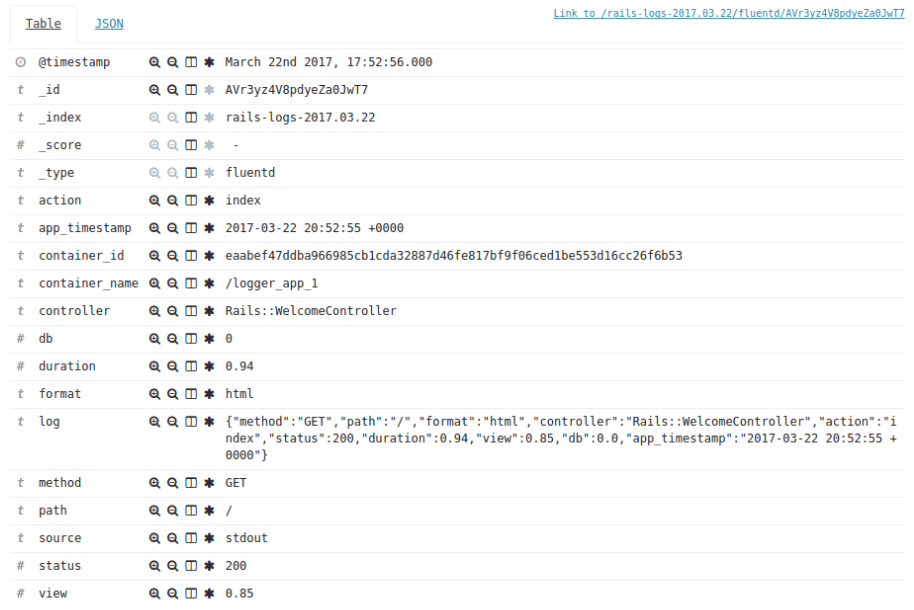
\includegraphics[width=\linewidth]{src/images/05-capitulo-5/kibana-logs.png}
  \caption{Vista de logs de \gls{term:ror} en \gls{term:kibana}}
  \label{fig:kibana-logs}
\end{figure}

En la \autoref{fig:kibana-logs} vemos como se visualiza en \gls{term:kibana}
una línea de logs tomada de nuestras aplicaciones \gls{term:ror}. En la misma
se puede apreciar cómo logramos separar la información contenida en una única
línea de log en varias para poder realizar consultas.

Ya tenemos \gls{term:kibana} configurado para poder comenzar a explorar los
logs almacenados en \gls{term:elasticsearch}. En la próxima sección contaremos
cómo configurar \gls{term:grafana}.
